\documentclass[11pt]{article}

\usepackage[margin=1.05in]{geometry}
\usepackage{amsmath,amssymb,amsthm}
\usepackage{mathtools}
\usepackage{graphicx}
\usepackage{booktabs}
\usepackage{array}
\usepackage{microtype}
\usepackage{tikz}
\usepackage[shortlabels]{enumitem}
\usepackage[colorlinks=true,linkcolor=blue!45!black,citecolor=blue!45!black,urlcolor=blue!45!black]{hyperref}

% ---------- colors for the two maps ----------
\definecolor{fred}{RGB}{178,58,46}
\definecolor{gblue}{RGB}{51,96,143}

% ---------- theorem environments ----------
\newtheorem{theorem}{Theorem}[section]
\newtheorem{lemma}[theorem]{Lemma}
\newtheorem{proposition}[theorem]{Proposition}
\newtheorem{corollary}[theorem]{Corollary}
\theoremstyle{definition}
\newtheorem{definition}[theorem]{Definition}
\newtheorem{example}[theorem]{Example}
\theoremstyle{remark}
\newtheorem{remark}[theorem]{Remark}
\newtheorem*{thmA}{Theorem A}
\newtheorem*{thmB}{Theorem B}
\newtheorem*{thmC}{Theorem C}

% ---------- notation macros ----------
\newcommand{\Q}{\mathbb{Q}}
\newcommand{\Z}{\mathbb{Z}}
\newcommand{\N}{\mathbb{N}}
\newcommand{\Qpos}{\Q_{>0}}
\newcommand{\Qneg}{\Q_{<0}}
\newcommand{\hj}[1]{[#1]^{-}}                 % negative (HJ) continued fraction
\newcommand{\lang}{\mathcal{L}}

% tree figure styles
\tikzset{
  vpos/.style={draw=fred,fill=fred!8,rounded corners=2.5pt,inner xsep=2.5pt,inner ysep=2pt},
  vneg/.style={draw=gblue,fill=gblue!8,rounded corners=2.5pt,inner xsep=2.5pt,inner ysep=2pt},
  vroot/.style={draw=black!70,fill=black!6,rounded corners=2.5pt,inner xsep=2.5pt,inner ysep=2pt},
  rk/.style={font=\tiny,text=black!55},
  ef/.style={draw=fred!75,thick},
  eg/.style={draw=gblue!75,thick},
  st/.style={circle,draw,minimum size=11mm,inner sep=0pt,font=\small},
}

\title{The tree of rationals generated by $x\mapsto x+1$ and $x\mapsto -1/x$:\\
 an exact distance formula and the rank recurrence\\[1ex]
 \large A solution to Problem 137 of Kagey's Open Problem Collection}
\author{Arjun Pemmasani}
\date{August 2026}

\begin{document}
\maketitle

\begin{abstract}
Starting from $0$ and repeatedly applying $f(x)=x+1$ and $g(x)=-1/x$ produces every rational
number. Sorting the rationals by the least number of applications needed to produce them gives
the tree in OEIS A226247/A226248; the set of rationals first reached in exactly $n$ steps is the
\emph{$n$-th rank}, with $a(n)$ elements. Problem 137 of Kagey's Open Problem Collection asks 3
questions: whether $a(n)=a(n-1)+a(n-3)$ for all $n\ge 4$, whether the vertices reached last by
$g$ are exactly the negative rationals, and whether the rank-$n$ rationals can be characterized.

We answer all 3. The central result is an exact formula for the rank $d(x)$ of every rational
$x$: iterating the \emph{parent map} $P(x)=x-1$ (for $x>0$), $P(x)=-1/x$ (for $x<0$) reaches $0$
in exactly $d(x)$ steps. Equivalently, if $x>0$ has negative (Hirzebruch--Jung) continued
fraction expansion $x=\hj{c_1,\dots,c_k}$ then $d(x)=c_1+\dots+c_k+k-1$, and $d(x)=d(-1/x)+1$
for $x<0$; a third form uses the ordinary continued fraction. From the formula, the tree has a
unique-parent structure with generating function $(1+t^2-t^3)/(1-t-t^3)$, so the recurrence
holds for all $n\ge4$ and fails only at $n=3$; a vertex is reached last by $g$ if and only if
it is negative; and rank $n$ is enumerated by integer compositions. This also completes the
transfer-matrix argument in the accepted Math.SE answer to the problem, which counted a language
of words but did not prove that words match rationals one to one.
\end{abstract}

\section{Introduction}\label{sec:intro}

In 2013 Kimberling \cite{oeisA226247} observed that the rational numbers can be generated from $0$ by the
two maps
\[
f(x)=x+1, \qquad g(x)=-\frac1x ,
\]
and organized them into generations: generation $1$ is $(0)$; from each already-generated value $c$ one
forms $c+1$ and (for $c\neq0$) $-1/c$, and generation $n+1$ consists of the values so formed from
generation $n$ that have not appeared before.  The resulting array is recorded in OEIS entries A226247
(denominators) and A226248 (numerators) \cite{oeisA226247,oeisA226248}.  That \emph{every} rational
eventually appears is classical in spirit: $f$ and $g$ generate the modular group
$\mathrm{PSL}_2(\Z)\cong C_2 * C_3$ acting on the projective rational line
\cite{serre1980,alperin1993}. We reprove it directly (Theorem~\ref{thm:dist}).

Writing $a(n)$ for the number of rationals appearing at the $n$-th step (with $a(0)=1$ for the root $0$),
the observed values
\[
1,\;1,\;2,\;2,\;3,\;5,\;7,\;10,\;15,\;22,\;32,\;47,\;69,\;101,\;\dots
\]
suggest the recurrence $a(n)=a(n-1)+a(n-3)$.  Kimberling's entry asserts (without proof) that these counts
form OEIS A097333 \cite{oeisA097333}; Kagey raised the question on Mathematics Stack Exchange in April 2025
\cite{kagey-mse} and lists it, together with two companion questions, as Problem 137 of his Open Problem
Collection \cite{kagey137}:

\begin{itemize}[leftmargin=2.2em]
\item[\textbf{Q1.}] Is $a(n)=a(n-1)+a(n-3)$ for all $n\ge4$?
\item[\textbf{Q2.}] Color a vertex \textcolor{gblue}{blue} if the last map applied to reach it is $g$, and
\textcolor{fred}{red} if it is $f$.  Is a vertex blue if and only if its value is negative?
\item[\textbf{Q3.}] Is there a way to characterize the rank-$n$ rational numbers?
\end{itemize}

The accepted answer to \cite{kagey-mse}, by the user mathmasterzach \cite{mmz}, made substantial progress on
Q1: using the relations $g^2=\mathrm{id}$ and $(g\circ f)^3=\mathrm{id}$ it observed that minimal-length
words in $f,g$ must avoid certain patterns, counted the words avoiding those patterns by a $14$-state
transfer matrix, and obtained precisely the generating function $(1+t^2-t^3)/(1-t-t^3)$.  What that argument
does not establish is that counting \emph{words} is the same as counting \emph{rationals}: it is not shown
that every pattern-avoiding word is in fact a minimal word for its endpoint, nor that distinct
pattern-avoiding words produce distinct rationals, nor that every rational is realized.  These are exactly
the difficult points, and the present paper supplies them.  Our main tool is an explicit formula for the
rank of an individual rational, which seems to be of independent interest and answers Q3 in a strong form.

Throughout, $d(x)$ denotes the rank of $x$: the least number of applications of $f,g$ producing $x$ from
$0$ (Definition~\ref{def:dist}).  Rationals are always written in lowest terms $p/q$ with $q\ge1$.

\begin{thmA}[= Theorem~\ref{thm:main}]
Let $a(n)$ be the number of rationals of rank $n$.  Then
\[
\sum_{n\ge0}a(n)\,t^n \;=\; \frac{1+t^2-t^3}{1-t-t^3}.
\]
Consequently $a(n)=a(n-1)+a(n-3)$ holds for every $n\ge4$, and fails at $n=3$ (where
$a(3)-a(2)-a(0)=-1$), so the bound $n\ge 4$ is sharp.  Moreover $a(n)=\mathrm{A097333}(n-1)$ for $n\ge1$,
the number of \emph{positive} rationals of rank $n$ is the Narayana's-cows number $\mathrm{A000930}(n-1)$,
and
\[
a(n)\;=\;C\,\psi^{\,n}+O\!\left(\psi^{-n/2}\right),\qquad
C=\frac{\psi^2+\psi}{\psi^2+3}=0.7019310679\ldots,
\]
where $\psi=1.4655712318\ldots$ (the ``supergolden ratio'') is the real root of $\psi^3=\psi^2+1$.
\end{thmA}

\begin{thmB}[= Theorems~\ref{thm:dist}, \ref{thm:hj} and \ref{thm:reg}]
Define the parent map $P(x)=x-1$ for $x>0$ and $P(x)=-1/x$ for $x<0$.  Then for every rational $x$ the
iteration of $P$ reaches $0$, and $d(x)$ equals the number of steps required.  Explicitly:
\begin{enumerate}[(i)]
\item $d(0)=0$, and $d(x)=d(-1/x)+1$ for $x<0$;
\item if $x>0$ has negative continued fraction expansion
$x=\hj{c_1,\dots,c_k}$ with $c_1\ge1$ and $c_2,\dots,c_k\ge2$ (Lemma~\ref{lem:hjexist}), then
\[
d(x)\;=\;c_1+c_2+\dots+c_k\;+\;k-1;
\]
\item if $x>0$ is written as the unique ordinary continued fraction $x=[b_0;b_1,\dots,b_m]$ with $m$
\emph{odd} (Lemma~\ref{lem:regstruct}), then
\[
d(x)\;=\;\sum_{i\;\mathrm{even}} b_i \;+\; 3\sum_{i\;\mathrm{odd}} b_i \;-\;2 .
\]
\end{enumerate}
In particular the rank-$n$ rationals are enumerated by integer compositions
(Corollary~\ref{cor:enum}), answering Q3.
\end{thmB}

\begin{thmC}[= Corollary~\ref{cor:tree}]
Every $x\neq0$ has exactly one neighbour closer to the root, namely $P(x)$, so the construction is a
well-defined tree in which no value is ever produced twice, even within a single generation.  The edge into
$x$ is an $f$-edge exactly when $x>0$ and a $g$-edge exactly when $x<0$; \emph{a vertex is blue if and only
if its value is negative} (answering Q2).  A vertex $x>0$ has two children ($x+1$ and $-1/x$); a vertex
$-1<x<0$ has one child ($x+1$); a vertex $x\le-1$ is a leaf, and for $x<-1$ the value $x+1$ is not new but
appeared exactly \emph{three} ranks earlier.
\end{thmC}

The ``three ranks earlier'' phenomenon is the combinatorial source of the summand $a(n-3)$; we will see that
it is a direct shadow of the relation $(gf)^3=\mathrm{id}$ in $\mathrm{PSL}_2(\Z)$.

\begin{figure}[t]
\centering
\resizebox{\textwidth}{!}{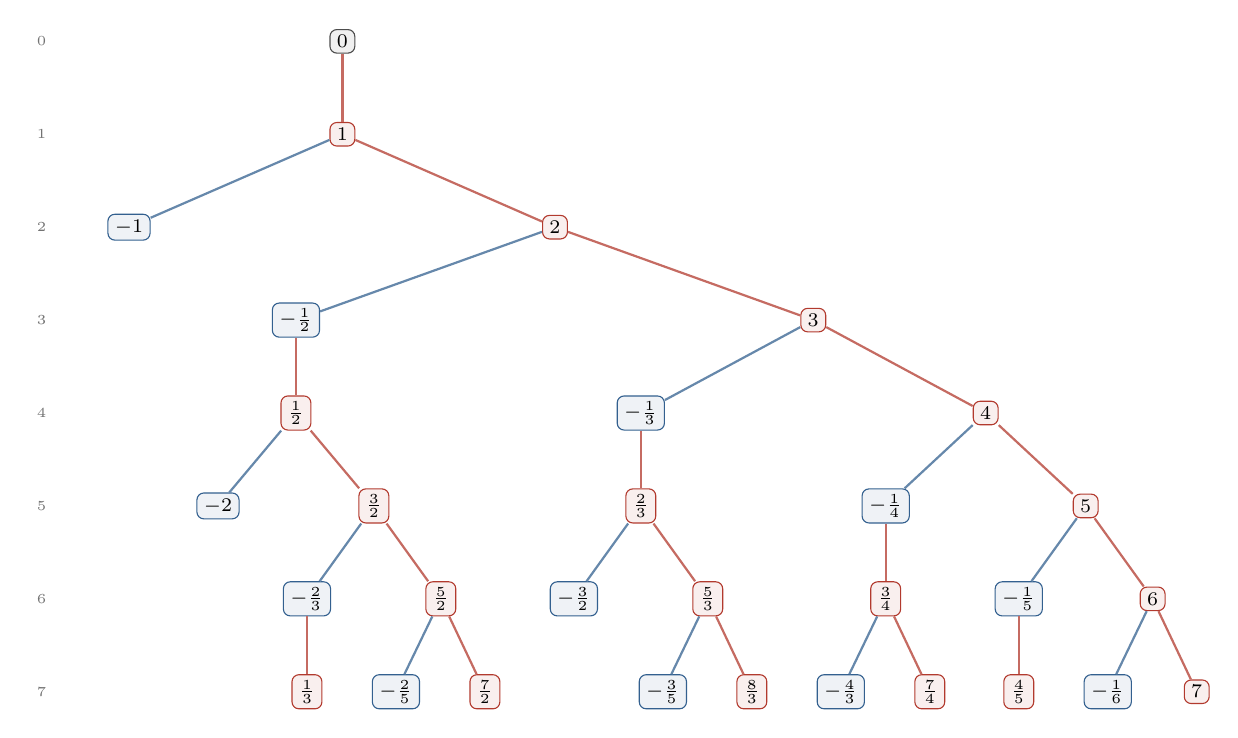
\begin{tikzpicture}[every node/.style={font=\scriptsize}]
\node[vroot] (n0_1) at (3.27,0.00) {$0$};
\node[vpos] (n1_1) at (3.27,-1.18) {$1$};
\node[vneg] (nm1_1) at (0.56,-2.36) {$-1$};
\node[vpos] (n2_1) at (5.97,-2.36) {$2$};
\node[vneg] (nm1_2) at (2.68,-3.54) {$-\tfrac{1}{2}$};
\node[vpos] (n3_1) at (9.25,-3.54) {$3$};
\node[vpos] (n1_2) at (2.68,-4.72) {$\tfrac{1}{2}$};
\node[vneg] (nm1_3) at (7.06,-4.72) {$-\tfrac{1}{3}$};
\node[vpos] (n4_1) at (11.44,-4.72) {$4$};
\node[vneg] (nm2_1) at (1.69,-5.90) {$-2$};
\node[vpos] (n3_2) at (3.67,-5.90) {$\tfrac{3}{2}$};
\node[vpos] (n2_3) at (7.06,-5.90) {$\tfrac{2}{3}$};
\node[vneg] (nm1_4) at (10.17,-5.90) {$-\tfrac{1}{4}$};
\node[vpos] (n5_1) at (12.71,-5.90) {$5$};
\node[vneg] (nm2_3) at (2.82,-7.08) {$-\tfrac{2}{3}$};
\node[vpos] (n5_2) at (4.52,-7.08) {$\tfrac{5}{2}$};
\node[vneg] (nm3_2) at (6.21,-7.08) {$-\tfrac{3}{2}$};
\node[vpos] (n5_3) at (7.91,-7.08) {$\tfrac{5}{3}$};
\node[vpos] (n3_4) at (10.17,-7.08) {$\tfrac{3}{4}$};
\node[vneg] (nm1_5) at (11.86,-7.08) {$-\tfrac{1}{5}$};
\node[vpos] (n6_1) at (13.56,-7.08) {$6$};
\node[vpos] (n1_3) at (2.82,-8.26) {$\tfrac{1}{3}$};
\node[vneg] (nm2_5) at (3.95,-8.26) {$-\tfrac{2}{5}$};
\node[vpos] (n7_2) at (5.08,-8.26) {$\tfrac{7}{2}$};
\node[vneg] (nm3_5) at (7.34,-8.26) {$-\tfrac{3}{5}$};
\node[vpos] (n8_3) at (8.47,-8.26) {$\tfrac{8}{3}$};
\node[vneg] (nm4_3) at (9.60,-8.26) {$-\tfrac{4}{3}$};
\node[vpos] (n7_4) at (10.73,-8.26) {$\tfrac{7}{4}$};
\node[vpos] (n4_5) at (11.86,-8.26) {$\tfrac{4}{5}$};
\node[vneg] (nm1_6) at (12.99,-8.26) {$-\tfrac{1}{6}$};
\node[vpos] (n7_1) at (14.12,-8.26) {$7$};
\node[rk] at (-0.55,0.00) {0};
\node[rk] at (-0.55,-1.18) {1};
\node[rk] at (-0.55,-2.36) {2};
\node[rk] at (-0.55,-3.54) {3};
\node[rk] at (-0.55,-4.72) {4};
\node[rk] at (-0.55,-5.90) {5};
\node[rk] at (-0.55,-7.08) {6};
\node[rk] at (-0.55,-8.26) {7};
\draw[ef] (n0_1) -- (n1_1);
\draw[eg] (n1_1) -- (nm1_1);
\draw[ef] (n1_1) -- (n2_1);
\draw[eg] (n2_1) -- (nm1_2);
\draw[ef] (n2_1) -- (n3_1);
\draw[eg] (n3_1) -- (nm1_3);
\draw[ef] (n3_1) -- (n4_1);
\draw[ef] (nm1_2) -- (n1_2);
\draw[eg] (n4_1) -- (nm1_4);
\draw[ef] (n4_1) -- (n5_1);
\draw[ef] (nm1_3) -- (n2_3);
\draw[eg] (n1_2) -- (nm2_1);
\draw[ef] (n1_2) -- (n3_2);
\draw[eg] (n5_1) -- (nm1_5);
\draw[ef] (n5_1) -- (n6_1);
\draw[ef] (nm1_4) -- (n3_4);
\draw[eg] (n2_3) -- (nm3_2);
\draw[ef] (n2_3) -- (n5_3);
\draw[eg] (n3_2) -- (nm2_3);
\draw[ef] (n3_2) -- (n5_2);
\draw[eg] (n6_1) -- (nm1_6);
\draw[ef] (n6_1) -- (n7_1);
\draw[ef] (nm1_5) -- (n4_5);
\draw[eg] (n3_4) -- (nm4_3);
\draw[ef] (n3_4) -- (n7_4);
\draw[eg] (n5_3) -- (nm3_5);
\draw[ef] (n5_3) -- (n8_3);
\draw[eg] (n5_2) -- (nm2_5);
\draw[ef] (n5_2) -- (n7_2);
\draw[ef] (nm2_3) -- (n1_3);
\end{tikzpicture}}
\caption{Ranks $0$--$7$ of the tree.  \textcolor{fred}{Red} edges apply $f(x)=x+1$; \textcolor{gblue}{blue}
edges apply $g(x)=-1/x$.  Every positive vertex is entered by an $f$-edge and every negative vertex by a
$g$-edge (Theorem C).  Vertices $\le-1$ are leaves.  Row numbers on the left are ranks; the rows agree with
Kimberling's generations \cite{oeisA226247} (his generation $j$ is rank $j-1$).}
\label{fig:tree}
\end{figure}

\paragraph{Plan of the paper.}
Section~\ref{sec:setup} fixes notation and shows that the several definitions of ``rank'' in the sources
(Kimberling's generations, Kagey's figure, the sets $X_n$ of \cite{kagey-mse}) agree.
Section~\ref{sec:parent} introduces the parent map and proves the distance formula
(Theorem~\ref{thm:dist}), from which the tree structure and the answer to Q2 follow.
Section~\ref{sec:cf} converts the formula into the two continued-fraction forms and answers Q3.
Section~\ref{sec:count} counts, proving Theorem A.  Section~\ref{sec:words} describes the geodesic words,
proves that they form exactly the regular language counted in \cite{mmz}, and thereby completes that
argument.  Section~\ref{sec:verify} reports the computational verification.  Section~\ref{sec:remarks}
collects further remarks.  The paper is self-contained; the references are context, not dependencies.

\section{Setup: the graph, ranks, and generations}\label{sec:setup}

\begin{definition}\label{def:dist}
Let $G$ be the directed graph with vertex set $\Q$ and, for every $x\in\Q$, an \emph{$f$-edge}
$x\to x+1$, and for every $x\in\Q\setminus\{0\}$, a \emph{$g$-edge} $x\to-1/x$.  (There is no $g$-edge out
of $0$, matching the fact that $g(0)$ is undefined.)  For $x\in\Q$ let
\[
d(x)\;=\;\text{length of a shortest directed path from $0$ to $x$ in }G \;\in\;\Z_{\ge0}\cup\{\infty\},
\]
and call $d(x)$ the \emph{rank} of $x$.  Equivalently, $d(x)$ is the least $n$ such that some sequence of
$n$ applications of $f$ and $g$, each application being defined, transforms $0$ into $x$.  We write
\[
X_n=\{x\in\Q:\ d(x)=n\},\qquad a(n)=|X_n| ,
\]
adopting the notation of \cite{kagey-mse}.  Theorem~\ref{thm:dist} will show $d(x)<\infty$ for all $x$.
\end{definition}

Note that $d(0)=0$ and that $X_0=\{0\}$: the empty path is the only path of length $0$.

Kimberling's construction \cite{oeisA226247} builds rows: row $1$ is $(0)$; given row $n$ with entries
$(c_1,\dots,c_z)$, row $n+1$ is obtained from the vector
$\left(c_1+1,\ -1/c_1,\ c_2+1,\ -1/c_2,\ \dots\right)$ (omitting $-1/c_i$ when $c_i=0$) by deleting values
generated in rows $1,\dots,n$.  The following proposition shows this is breadth-first search, so his rows,
Kagey's ranks \cite{kagey137}, and the sets $X_n$ all agree.

\begin{proposition}[generations are metric spheres]\label{prop:rows}
For every $n\ge0$, the set of values in Kimberling's row $n+1$ equals $X_n$.
\end{proposition}

\begin{proof}
Induction on $n$; the case $n=0$ is the definition.  Assume rows $1,\dots,n$ carry exactly the values in
$X_0,\dots,X_{n-1}$.  If $y$ lies in row $n+1$, then $y$ is an out-neighbour in $G$ of some $x\in X_{n-1}$,
so $d(y)\le d(x)+1=n$; and $y$ survived deletion, so $y\notin X_0\cup\dots\cup X_{n-1}$, i.e.\ $d(y)\ge n$.
Hence $y\in X_n$.  Conversely let $y\in X_n$ with $n\ge1$ and let $x$ be the predecessor of $y$ on a
shortest path from $0$.  A prefix of a shortest path is a shortest path, so $d(x)=n-1$, i.e.\ $x$ lies in
row $n$; thus $y$ is listed in the vector forming row $n+1$, and $y$ is not deleted since $d(y)=n$.
\end{proof}

\begin{remark}\label{rem:dupes}
One point requires care.  A value $y$ could conceivably be listed \emph{twice} in the vector forming row
$n+1$, once as $c+1$ and once as $-1/c'$ for two different entries $c,c'$ of row $n$, and the
construction as stated does not say whether such a duplicate is deleted.  Corollary~\ref{cor:tree}(a) shows
that this situation never occurs: each $y\neq0$ has exactly one in-neighbour at rank $d(y)-1$.  So the rows
are duplicate-free and $|$row $n+1|=a(n)$ unambiguously.  (Our computational check of
Section~\ref{sec:verify} confirms agreement with the published A226247/A226248 data, including the order of
entries within rows.)
\end{remark}

\paragraph{Words.}
It is convenient to speak of paths as words.  A \emph{word} is a finite string over the alphabet
$\{f,g\}$, written left to right in the order the maps are applied: the word $fg$ sends
$0\mapsto f(0)=1\mapsto g(1)=-1$.  (In composition notation the word $\ell_1\ell_2\cdots\ell_j$ is the map
$\ell_j\circ\dots\circ\ell_1$.)  A word is \emph{admissible at $0$} if every application along the way is
defined, i.e.\ $g$ is never applied to the value $0$; admissible words are exactly the directed paths of
$G$ starting at $0$, and $d(x)$ is the least length of an admissible word with endpoint $x$.

\section{The parent map and the exact distance formula}\label{sec:parent}

The key step is to find, for each $x$, a canonical shortest path from $0$ to $x$. From the small
cases (Figure~\ref{fig:tree}), the guess is that the last step into a positive vertex is always the
$f$-edge from $x-1$, and the last step into a negative vertex is always the $g$-edge from $-1/x$.
Undoing the guessed last step gives a candidate ``parent'' of each vertex, and iterating the parent
should walk back to the root. We now prove exactly that.

\begin{definition}\label{def:parent}
The \emph{parent map} $P:\Q\setminus\{0\}\to\Q$ is
\[
P(x)=
\begin{cases}
x-1, & x>0,\\[2pt]
-1/x, & x<0 .
\end{cases}
\]
\end{definition}

Observe that $P$ undoes an edge of $G$: for every $x\neq0$ there is an edge $P(x)\to x$, namely the
$f$-edge $(x-1)\to x$ when $x>0$, and the $g$-edge $(-1/x)\to x$ when $x<0$ (legal because $-1/x\neq0$).

\begin{lemma}[termination]\label{lem:term}
For every $x\in\Q$ the iteration $x,\,P(x),\,P^2(x),\dots$ reaches $0$ after finitely many steps.
\end{lemma}

\begin{proof}
First let $x>0$.  Successive subtractions of $1$ reach, after exactly $\lceil x\rceil$ steps, the value
$x-\lceil x\rceil$, which is $0$ if $x\in\Z$ and otherwise lies in the interval $(-1,0)$.  Next, if
$z\in(-1,0)$, write $z=-r/q$ in lowest terms with $0<r<q$; then $P(z)=-1/z=q/r>1$ is positive, in lowest
terms, with denominator $r<q$.

Now induct on the denominator $q\ge1$ of $x$, over all $x\in\Qpos\cup(-1,0)$.  If $q=1$: elements of
$(-1,0)$ with denominator $1$ do not exist, and a positive integer $x$ reaches $0$ after $x$ steps.  If
$q\ge2$ and $x>0$: $x$ is not an integer, so its orbit reaches a point of $(-1,0)$ with the same
denominator $q$, whose next iterate is positive with denominator $<q$; conclude by the induction
hypothesis.  If $q\ge2$ and $x\in(-1,0)$: $P(x)$ is positive with denominator $<q$, and again the induction
hypothesis applies.

Finally, a negative $x\notin(-1,0)$ (that is, $x\le-1$) has $P(x)=-1/x>0$, reducing to the positive case;
and $x=0$ is trivial.
\end{proof}

\begin{definition}\label{def:D}
For $x\in\Q$ let $D(x)$ be the number of steps in which the $P$-orbit of $x$ reaches $0$.  Thus $D(0)=0$
and
\begin{equation}\label{eq:Drec}
D(x)=D(P(x))+1 \qquad (x\neq0),
\end{equation}
and $D$ is determined by these two properties.  More precisely:
\end{definition}

\begin{lemma}[uniqueness principle]\label{lem:unique}
If $F:\Q\to\Z_{\ge0}$ satisfies $F(0)=0$ and $F(x)=F(P(x))+1$ for all $x\neq0$, then $F=D$.
\end{lemma}

\begin{proof}
By Lemma~\ref{lem:term} the orbit $x,P(x),\dots,P^{D(x)}(x)=0$ is finite; unwinding the recursion along it
gives $F(x)=D(x)+F(0)=D(x)$.
\end{proof}

The next lemma computes how $D$ changes along \emph{all four} edge types of $G$, not only the two that $P$
undoes.  Items (D1)--(D3) are immediate; (D4) is the crucial computation.

\begin{lemma}[increment identities]\label{lem:incr}
For all $x\in\Q$:
\begin{enumerate}[label={(D\arabic*)}]
\item if $x>0$, then $D(x)=D(x-1)+1$;
\item if $x<0$, then $D(x)=D(-1/x)+1$;
\item if $x>0$, then $D(-1/x)=D(x)+1$;
\item if $x<0$, then $D(x-1)=D(x)+3$.
\end{enumerate}
\end{lemma}

\begin{proof}
(D1) and (D2) restate \eqref{eq:Drec}.  For (D3): $-1/x<0$, so (D2) applied to $-1/x$ gives
$D(-1/x)=D\!\left(-\tfrac{1}{-1/x}\right)+1=D(x)+1$.

For (D4), put $z=x-1$; since $x<0$ we have $z<-1$.  We follow the orbit of $z$ for four steps, at each step
checking the sign to see which branch of $P$ applies:
\[
z \;\xmapsto{\;P\;}\; \frac{1}{1-x}
\;\xmapsto{\;P\;}\; \frac{x}{1-x}
\;\xmapsto{\;P\;}\; 1-\frac1x
\;\xmapsto{\;P\;}\; -\frac1x \;=\;P(x).
\]
Indeed: $z<0$, so $P(z)=-1/z=1/(1-x)$, which lies in $(0,1)$ because $1-x>1$; hence
$P^2(z)=\tfrac{1}{1-x}-1=\tfrac{x}{1-x}$, which is negative (and lies in $(-1,0)$, being $-u/(1+u)$ with
$u=-x>0$); hence $P^3(z)=-\tfrac{1-x}{x}=1-\tfrac1x$, which exceeds $1$ because $-1/x>0$; hence
$P^4(z)=-\tfrac1x$, which is $P(x)$ because $x<0$.  Therefore
$D(z)=4+D(P(x))=4+\bigl(D(x)-1\bigr)=D(x)+3$.
\end{proof}

\begin{remark}\label{rem:relation}
Read backwards, the computation in (D4) exhibits the path
\[
-\tfrac1x \xrightarrow{\,f\,} 1-\tfrac1x \xrightarrow{\,g\,} \tfrac{x}{1-x}
\xrightarrow{\,f\,} \tfrac{1}{1-x} \xrightarrow{\,g\,} x-1 ,
\]
i.e.\ $x-1=(g\circ f\circ g\circ f\circ g)(x)$: this is exactly the relation
$f^{-1}=g\circ f\circ g\circ f\circ g$ quoted in \cite{kagey137}, equivalently $(g\circ f)^3=\mathrm{id}$,
which together with $g^2=\mathrm{id}$ presents $\mathrm{PSL}_2(\Z)\cong C_2*C_3$
\cite{serre1980,alperin1993}.  The $3$ in (D4), five letters of the relator minus the cancellation $g\cdot g=\mathrm{id}$, is
exactly where the $t^3$ of Theorem A will come from. The proof above is a direct check and uses no
group theory.
\end{remark}

\begin{theorem}[exact distance formula, dynamic form]\label{thm:dist}
Every rational is reachable from $0$ in $G$, and $d(x)=D(x)$ for all $x\in\Q$.
\end{theorem}

\begin{proof}
\emph{Upper bound $d\le D$.}
The reversed $P$-orbit $\;0=P^{D(x)}(x),\;P^{D(x)-1}(x),\;\dots,\;P(x),\;x\;$ is a directed path in $G$,
because each consecutive pair $(P(y),y)$ is an edge (observation after Definition~\ref{def:parent}).  Its
length is $D(x)$, so $x$ is reachable and $d(x)\le D(x)$.

\emph{Lower bound $d\ge D$.}
We first check that
\begin{equation}\label{eq:bellman}
D(x)\le D(y)+1 \qquad\text{for every edge } y\to x \text{ of } G .
\end{equation}
There are five cases.
\begin{itemize}
\item $f$-edge into $x>0$: here $y=x-1$ and (D1) gives $D(x)=D(y)+1$.
\item $f$-edge into $x=0$: here $y=-1$, and $D(0)=0\le D(-1)+1$.
\item $f$-edge into $x<0$: here $y=x-1$ and (D4) gives $D(x)=D(y)-3\le D(y)+1$.
\item $g$-edge into $x<0$: here $y=-1/x$ and (D2) gives $D(x)=D(y)+1$.
\item $g$-edge into $x>0$: here $y=-1/x<0$, and (D3) gives $D(y)=D(x)+1$, i.e.\ $D(x)=D(y)-1$.
\end{itemize}
(There is no $g$-edge into $0$.)  Now induct on $n=d(x)$.  For $n=0$, $x=0$ and $D(0)=0$.  For $n\ge1$,
let $y\to x$ be the final edge of a shortest path; then $d(y)=n-1$, so by induction $D(y)\le d(y)$, and
\eqref{eq:bellman} gives $D(x)\le D(y)+1\le d(y)+1=d(x)$.
\end{proof}

From now on we use $d$ and $D$ interchangeably.  The next two corollaries unpack
Theorem~\ref{thm:dist} into the local structure of the tree; together they prove Theorem C.

\begin{corollary}[in-neighbour distances]\label{cor:innbr}
Let $x\neq0$.  The in-neighbours of $x$ in $G$ are exactly $x-1$ (via $f$) and $-1/x$ (via $g$), and their
ranks are:
\begin{center}
\begin{tabular}{c c c}
\toprule
 & \emph{in-neighbour } $x-1$ & \emph{in-neighbour } $-1/x$\\
\midrule
$x>0$ & $d(x)-1$ & $d(x)+1$\\
$x<0$ & $d(x)+3$ & $d(x)-1$\\
\bottomrule
\end{tabular}
\end{center}
In particular exactly one in-neighbour of $x$ is closer to the root than $x$, namely $P(x)$.
\end{corollary}

\begin{proof}
The in-neighbours are as listed because $f^{-1}(x)=x-1$ always exists and $g(y)=x$ has the unique solution
$y=-1/x$.  The table restates (D1)--(D4) via Theorem~\ref{thm:dist}.  (Note $x-1\neq-1/x$ for rational $x$,
since $x^2-x+1$ has no rational root, so the two in-neighbours are distinct.)
\end{proof}

\begin{corollary}[tree structure; answers Q2]\label{cor:tree}
\begin{enumerate}[(a)]
\item Each $x\neq0$ is produced, at stage $d(x)$, by exactly one element of $X_{d(x)-1}$, namely its parent
$P(x)$.  Consequently no value is ever produced twice, not even twice within one generation, and the
construction is a well-defined rooted tree, independent of any tie-breaking convention.
\item The edge entering $x$ is an $f$-edge exactly when $x>0$ and a $g$-edge exactly when $x<0$.  With the
coloring of Q2: \emph{a vertex is blue if and only if its value is negative} (the root is uncolored).
\item Children: a vertex $x>0$ has exactly the two children $x+1$ and $-1/x$; a vertex $x\in(-1,0)$ has
exactly the one child $x+1\in(0,1)$; every vertex $x\le-1$ is a leaf.  Moreover for $x<-1$ the blocked
value $x+1$ is not new but \emph{three ranks old}: $d(x+1)=d(x)-3$; and for $x=-1$ the blocked value
$x+1=0$ is the root.
\end{enumerate}
\end{corollary}

\begin{proof}
(a) An element $y$ of the vector forming generation $d(y)+1$ is produced once for each of its in-neighbours
lying in $X_{d(y)-1}$; by Corollary~\ref{cor:innbr} there is exactly one such in-neighbour, $P(y)$.

(b) The unique parent edge is the $f$-edge from $x-1$ when $x>0$ and the $g$-edge from $-1/x$ when $x<0$.

(c) Let $x>0$.  Its out-neighbours are $x+1$ and $-1/x$; by (D1) applied to $x+1$ and by (D3), both have
rank $d(x)+1$, so both are children.  Let $x\in(-1,0)$.  Then $x+1\in(0,1)$ is positive, and (D1) applied
to $x+1$ gives $d(x+1)=d(x)+1$, a child; while $-1/x$ is the parent (rank $d(x)-1$).  Let $x<-1$.  Then
$-1/x$ is the parent; and since $x=(x+1)-1$ with $x+1<0$, identity (D4) applied to the negative number
$x+1$ yields $d(x)=d(x+1)+3$, i.e.\ $d(x+1)=d(x)-3$: three ranks old, so not a child.  Finally $x=-1$ has out-neighbours $0$ (the root) and $1$ (its
parent), so it is a leaf.
\end{proof}

\begin{example}\label{ex:orbit}
Take $x=-\tfrac72$.  The $P$-orbit is
\[
-\tfrac72 \to \tfrac27 \to -\tfrac57 \to \tfrac75 \to \tfrac25 \to -\tfrac35 \to \tfrac53 \to \tfrac23
\to -\tfrac13 \to 3 \to 2 \to 1 \to 0,
\]
so $d(-7/2)=12$.  Reversing the orbit gives the canonical geodesic word $fffgffgffgfg$
(apply $f,f,f,g,f,f,g,f,f,g,f,g$ in this order to $0$).
\end{example}

\section{Continued-fraction forms of the distance formula}\label{sec:cf}

Iterating $P$ from a positive rational performs ceiling-type division: it subtracts $\lceil x\rceil$ ones,
then flips.  This is precisely the algorithm computing the \emph{negative} (or Hirzebruch--Jung, or
``minus'') continued fraction expansion \cite{hirzebruch1953,popescu2007}, which makes the orbit length
computable in closed form.  We prove what we need from scratch.

\begin{definition}
For integers $c_1,\dots,c_k$ define, when the right sides are defined and nonzero where required,
\[
\hj{c_1}=c_1, \qquad
\hj{c_1,c_2,\dots,c_k}=c_1-\cfrac{1}{\hj{c_2,\dots,c_k}} .
\]
\end{definition}

\begin{lemma}[existence and uniqueness of the expansion]\label{lem:hjexist}
Every rational $x>0$ has exactly one representation
\[
x=\hj{c_1,c_2,\dots,c_k},\qquad k\ge1,\ \ c_1\ge1,\ \ c_i\ge2\ (2\le i\le k),
\]
and in it $c_1=\lceil x\rceil$.  Moreover every tail satisfies $\hj{c_j,\dots,c_k}>1$ for $j\ge2$.
\end{lemma}

\begin{proof}
\emph{Existence.}  Run the algorithm: given $x>0$, emit $c=\lceil x\rceil$ and stop if $x=c$; otherwise
recurse on $x'=1/(c-x)$.  If $x=p/q$ in lowest terms is not an integer, then $c q-p\in\{1,\dots,q-1\}$ and
$x'=q/(cq-p)$, again in lowest terms (any common divisor of $q$ and $cq-p$ divides $p$), with denominator
$cq-p<q$; so the algorithm terminates.  Moreover $x'>1$, so every emitted digit after the first is
$\lceil x'\rceil\ge2$; and $c_1=\lceil x\rceil\ge1$ because $x>0$.  Unwinding $x=c-1/x'$ shows the emitted
digits satisfy $x=\hj{c_1,\dots,c_k}$.

\emph{Tails exceed $1$.}  By downward induction: $\hj{c_k}=c_k\ge2>1$; and if $y=\hj{c_{j+1},\dots,c_k}>1$
then $\hj{c_j,\dots,c_k}=c_j-1/y>c_j-1\ge1$.

\emph{Uniqueness.}  Suppose $x=\hj{c_1,\dots,c_k}$ is any representation obeying the digit conditions.  If
$k=1$ then $x=c_1\in\Z$.  If $k\ge2$ then $x=c_1-1/y$ with $y=\hj{c_2,\dots,c_k}>1$ by the previous
paragraph, so $x\in(c_1-1,c_1)$; in particular $x\notin\Z$, the digit $c_1$ is forced to be
$\lceil x\rceil$, and $y=1/(c_1-x)$ is determined.  Induction on $k$ finishes: an integer has only the
$k=1$ representation, and a non-integer has forced first digit and forced tail.
\end{proof}

\begin{theorem}[distance formula, negative-continued-fraction form]\label{thm:hj}
Let $x>0$ have the expansion of Lemma~\ref{lem:hjexist}.  Then
\[
d(x)=c_1+c_2+\dots+c_k+k-1 .
\]
Together with $d(0)=0$ and $d(x)=d(-1/x)+1$ for $x<0$ (identity (D2)), this determines $d$ on all
of $\Q$.
\end{theorem}

\begin{proof}
By Theorem~\ref{thm:dist} we may compute $D$.  Induct on $k$.  If $k=1$ then $x=c_1$ is a positive integer
and its orbit is $c_1$ subtractions.  If $k\ge2$: since $c_1=\lceil x\rceil$, the orbit performs $c_1$
subtractions, arriving at
\[
x-c_1=-\frac{1}{\hj{c_2,\dots,c_k}}\;\in\;(-1,0)
\]
(the membership because the tail exceeds $1$), then one flip, arriving at $\hj{c_2,\dots,c_k}$.  By the
induction hypothesis the remaining orbit takes $\bigl(\sum_{i\ge2}c_i\bigr)+(k-1)-1$ steps, for a total of
$c_1+1+\sum_{i\ge2}c_i+k-2=\sum_i c_i+k-1$.
\end{proof}

\begin{corollary}[explicit description of the ranks; answers Q3]\label{cor:enum}
For $n\ge1$,
\begin{align*}
X_n\cap\Qpos &= \Bigl\{\hj{c_1,\dots,c_k}\ :\ k\ge1,\ c_1\ge1,\ c_2,\dots,c_k\ge2,\
\textstyle\sum_i c_i=n+1-k\Bigr\},\\
X_n\cap\Qneg &= \Bigl\{-1/y\ :\ y\in X_{n-1}\cap\Qpos\Bigr\},
\end{align*}
and both descriptions are bijective parametrizations (distinct digit strings give distinct rationals, and
$y\mapsto-1/y$ is injective).  In particular rank $n$ is a finite set enumerated by integer compositions.
\end{corollary}

\begin{proof}
The first line combines Lemma~\ref{lem:hjexist} (each positive rational has exactly one digit string) with
Theorem~\ref{thm:hj} (the rank of the value of a digit string is its weight $\sum c_i+k-1$).  For the
second line: if $x<0$ then $-1/x>0$ and (D2) gives $d(-1/x)=d(x)-1$; conversely if $y>0$ then $-1/y<0$ and
(D3) gives $d(-1/y)=d(y)+1$.  So $x\mapsto-1/x$ and $y\mapsto-1/y$ are mutually inverse bijections between
$X_n\cap\Qneg$ and $X_{n-1}\cap\Qpos$.
\end{proof}

\begin{example}\label{ex:rank5}
$n=5$: the digit strings of weight $5$ are $(5)$, $(1,3)$, $(2,2)$, with values $5$, $\hj{1,3}=\tfrac23$,
$\hj{2,2}=\tfrac32$; and the rank-$4$ positives are $4,\tfrac12$ (strings $(4)$, $(1,2)$), giving negatives
$-\tfrac14$, $-2$.  So $X_5=\{5,\tfrac23,\tfrac32,-\tfrac14,-2\}$, matching Figure~\ref{fig:tree}.
\end{example}

\begin{example}\label{ex:27}
$x=\tfrac27$: the algorithm gives $\tfrac27=\hj{1,2,2,3}$
(check: $\hj{3}=3$, $\hj{2,3}=\tfrac53$, $\hj{2,2,3}=\tfrac75$, $1-\tfrac57=\tfrac27$), so
$d(2/7)=(1+2+2+3)+4-1=11$ and $d(-7/2)=12$, agreeing with Example~\ref{ex:orbit}.
\end{example}

\subsection{The ordinary continued fraction form}

Recall the ordinary (regular) continued fraction notation
\[
[b_0;b_1,\dots,b_m]=b_0+\cfrac{1}{b_1+\cfrac{1}{\ddots+\cfrac{1}{b_m}}},
\qquad b_0\ge0,\ b_i\ge1\ (1\le i\le m),\ b_i\in\Z .
\]
We call $m$ the \emph{length}.  It is classical that a positive rational has exactly two such expansions
(see e.g.\ \cite[Ch.~X]{hardywright}); for self-containedness we prove the precise statement we use.

\begin{lemma}[odd-length normalization]\label{lem:regstruct}
\begin{enumerate}[(a)]
\item For a digit string as above with $m\ge1$, the value $v=[b_1;b_2,\dots,b_m]$ of the tail satisfies
$v>1$, except that $v=1$ exactly when $m=1$ and $b_1=1$.
\item Every rational $x>0$ has exactly one expansion $x=[b_0;b_1,\dots,b_m]$ of \emph{odd} length $m$.
\item In the odd-length expansion, $b_0\ge1$ if and only if $x>1$.
\end{enumerate}
\end{lemma}

\begin{proof}
(a) If $m=1$ then $v=b_1\ge1$ with equality iff $b_1=1$.  If $m\ge2$ then
$v=b_1+1/[b_2;\dots;b_m]>b_1\ge1$.

(b) \emph{Uniqueness.}  We show by strong induction on the denominator that for each parity class
$\varepsilon\in\{0,1\}$, $x$ has at most one expansion with $m\equiv\varepsilon\pmod 2$.  Let
$x=[b_0;b_1,\dots,b_m]$.  If $m=0$ then $x=b_0\in\Z$.  If $m\ge1$, write $x=b_0+1/v$ with
$v=[b_1;\dots,b_m]$.  By (a), either $v>1$, and then $x\in(b_0,b_0+1)$ is not an integer, $b_0=\lfloor
x\rfloor$ and $v=1/(x-b_0)$ are forced, and the tail is an expansion of $v$ of length $m-1$ (its leading
digit $b_1$ automatically satisfies $b_1\ge1$), or $(m,b_1)=(1,1)$ and $x=b_0+1\in\Z$.  So: for integer
$x\ge1$, the only expansions are $[x]$ (length $0$) and $[x-1;1]$ (length $1$), one per parity.  For
non-integer $x$, expansions of $x$ of length $m$ correspond bijectively to expansions of
$v=1/(x-\lfloor x\rfloor)>1$ of length $m-1$; since $v$ has smaller denominator than $x$, the induction
hypothesis (one per parity for $v$) gives one per parity for $x$.

\emph{Existence.}  The Euclidean algorithm produces one expansion; if its length has the wrong parity,
toggle using $[\,\dots,b_m]=[\,\dots,b_m-1,1]$ when $b_m\ge2$, or $[\,\dots,b_{m-1},1]=[\,\dots,b_{m-1}+1]$
when $b_m=1$, or $[x]=[x-1;1]$ for integers; each toggle changes the length by one.

(c) Since $m$ is odd, $m\ge1$, so $x=b_0+1/v$ with $v\ge1$.  If $b_0\ge1$ then $x>b_0\ge1$; if $b_0=0$
then $x=1/v\le1$ by (a).  Hence $b_0\ge1\iff x>1$.  (The borderline value $x=1$ has odd-length form
$[0;1]$.)
\end{proof}

\begin{lemma}[complement identity]\label{lem:compl}
Let $b\ge1$ and let $\mathrm{t}$ denote a (possibly empty) admissible tail, and put
$u=[b;\mathrm{t}]\ge1$.  Then
\[
[0;1,b,\mathrm{t}]=\frac{u}{1+u},\qquad [0;b+1,\mathrm{t}]=\frac{1}{1+u},
\]
and in particular $[0;1,b,\mathrm{t}]+[0;b+1,\mathrm{t}]=1$.
\end{lemma}

\begin{proof}
$[1;b,\mathrm{t}]=1+1/u=(1+u)/u$, so $[0;1,b,\mathrm{t}]=u/(1+u)$.  And
$[b+1;\mathrm{t}]=1+[b;\mathrm{t}]=1+u$, so $[0;b+1,\mathrm{t}]=1/(1+u)$.
\end{proof}

\begin{theorem}[distance formula, ordinary-continued-fraction form]\label{thm:reg}
Let $x>0$ and let $x=[b_0;b_1,\dots,b_m]$ be its unique odd-length expansion
(Lemma~\ref{lem:regstruct}).  Then
\[
d(x)\;=\;\sum_{i\ \mathrm{even}} b_i\;+\;3\sum_{i\ \mathrm{odd}} b_i\;-\;2 .
\]
\end{theorem}

\begin{proof}
Let $E(x)$ denote the right-hand side for $x>0$; extend $E$ to all of $\Q$ by $E(0)=0$ and
$E(x)=E(-1/x)+1$ for $x<0$.  By the uniqueness principle (Lemma~\ref{lem:unique}) it suffices to prove
$E(x)=E(P(x))+1$ for every $x\neq0$.  For $x<0$ this holds by definition.  Three cases remain for $x>0$.

\emph{Case $x>1$.}  By Lemma~\ref{lem:regstruct}(c), $b_0\ge1$, and $x-1=[b_0-1;b_1,\dots,b_m]$ is again a
valid odd-length expansion (the leading digit may drop to $0$); by uniqueness it is \emph{the} odd-length
expansion of $x-1$.  Only the even-position digit $b_0$ changed, so $E(x)=E(x-1)+1$.

\emph{Case $x=1$.}  $E(1)=E([0;1])=0+3\cdot1-2=1=E(0)+1$.

\emph{Case $0<x<1$.}  Here $b_0=0$, and $P(x)=x-1\in(-1,0)$, so
$E(x-1)=E\bigl(\tfrac{1}{1-x}\bigr)+1$ and we must show $E(x)=E\bigl(\tfrac{1}{1-x}\bigr)+2$.  Note
$m\ge1$; and if $b_1=1$ then $m\ge3$, since $[0;1]=1$ is excluded.  Apply Lemma~\ref{lem:compl}:
\begin{itemize}
\item If $b_1=1$: from $x=[0;1,b_2,\mathrm{t}]$ (tail $\mathrm{t}=b_3,\dots,b_m$) we get
$1-x=[0;b_2+1,\mathrm{t}]$, hence
\[
\tfrac{1}{1-x}=[\,b_2+1;\,b_3,\dots,b_m\,],
\]
a valid expansion of length $m-2$, still odd.  Compared with $x$'s digits, position $0$ gained $1$ (weight
$1$), the odd-position digit $b_1=1$ disappeared (weight $3$), and all other digits kept their position
parity (indices shifted by two).  Hence $E\bigl(\tfrac1{1-x}\bigr)=E(x)+1-3=E(x)-2$.
\item If $b_1\ge2$: from $x=[0;b_1,\mathrm{t}]=[0;(b_1-1)+1,\mathrm{t}]$ we get
$1-x=[0;1,b_1-1,\mathrm{t}]$, hence
\[
\tfrac{1}{1-x}=[\,1;\,b_1-1,\,b_2,\dots,b_m\,],
\]
a valid expansion of length $m$, odd.  Position $0$ gained $1$ and position $1$ lost $1$ (weight $3$); all
other digits are unchanged in place.  Hence again $E\bigl(\tfrac1{1-x}\bigr)=E(x)+1-3=E(x)-2$. \qedhere
\end{itemize}
\end{proof}

\begin{example}
$x=\tfrac27=[0;3,2]$ has odd-length form $[0;3,1,1]$, so
$d(2/7)=(0+1)+3(3+1)-2=11$, agreeing with Example~\ref{ex:27}.  Similarly $\tfrac35=[0;1,1,2]$ (already odd
length) gives $d(3/5)=(0+1)+3(1+2)-2=8$.
\end{example}

\section{Counting: proof of Theorem A}\label{sec:count}

\begin{theorem}[main count]\label{thm:main}
Let $r(n)=|X_n\cap\Qpos|$.  Then $a(0)=1$, $a(n)=r(n)+r(n-1)$ for $n\ge1$, and, as formal power series,
\[
R(t):=\sum_{n\ge1}r(n)\,t^n=\frac{t}{1-t-t^3},
\qquad
A(t):=\sum_{n\ge0}a(n)\,t^n=\frac{1+t^2-t^3}{1-t-t^3}.
\]
Consequently:
\begin{enumerate}[(a)]
\item $a(n)=a(n-1)+a(n-3)$ for every $n\ge4$;
\item the recurrence fails at $n=3$: $a(3)-a(2)-a(0)=-1$;
\item $r(n)=\mathrm{A000930}(n-1)$ \emph{(Narayana's cows)} and $a(n)=\mathrm{A097333}(n-1)$ for $n\ge1$.
\end{enumerate}
\end{theorem}

\begin{proof}
The decomposition $a(n)=r(n)+r(n-1)$ for $n\ge1$ is the bijection of Corollary~\ref{cor:enum} between
rank-$n$ negatives and rank-$(n-1)$ positives (and $0\in X_0$ only).

By Corollary~\ref{cor:enum}, $r(n)$ is the number of digit strings $(c_1,\dots,c_k)$, $c_1\ge1$,
$c_i\ge2$ $(i\ge2)$, of weight $\sum_ic_i+k-1=n$.  Attaching weight $t^{c_1}\prod_{i\ge2}t^{c_i+1}$ to a
string and summing,
\[
R(t)=\sum_{k\ge1}\Bigl(\sum_{c\ge1}t^{c}\Bigr)\Bigl(\sum_{c\ge2}t^{c+1}\Bigr)^{k-1}
=\frac{t}{1-t}\sum_{k\ge1}\Bigl(\frac{t^{3}}{1-t}\Bigr)^{k-1}
=\frac{t}{1-t}\cdot\frac{1}{1-\frac{t^3}{1-t}}
=\frac{t}{1-t-t^{3}} ,
\]
the geometric series being legitimate formally because $t^3/(1-t)$ has zero constant term.  Hence
\[
A(t)=1+R(t)+tR(t)=1+\frac{(1+t)t}{1-t-t^3}=\frac{(1-t-t^3)+t+t^2}{1-t-t^3}=\frac{1+t^2-t^3}{1-t-t^3},
\]
using $\sum_{n\ge1}r(n-1)t^n=tR(t)$ (note $r(0)=0$).  Multiplying out,
$(1-t-t^3)A(t)=1+t^2-t^3$; comparing coefficients of $t^n$:
\[
a(n)-a(n-1)-a(n-3)=[t^n]\bigl(1+t^2-t^3\bigr)=
\begin{cases}
0,& n\ge4,\\
-1,& n=3,
\end{cases}
\]
which proves (a) and (b) (indeed $a(3)=2$ while $a(2)+a(0)=3$).  For (c): A000930 has generating function
$1/(1-t-t^3)$ and A097333 has generating function $(1+t)/(1-t-t^3)$ \cite{oeisA000930,oeisA097333}, so
$R(t)=t\cdot\frac1{1-t-t^3}$ and $A(t)-1=t\cdot\frac{1+t}{1-t-t^3}$ give exactly the stated shifts.
\end{proof}

\begin{proposition}[asymptotics]\label{prop:asymp}
Let $\psi=1.4655712318\ldots$ be the real root of $\psi^3=\psi^2+1$.  Then
\[
a(n)=C\,\psi^{\,n}+O\!\bigl(\psi^{-n/2}\bigr),
\qquad
C=\frac{\psi^{2}+\psi}{\psi^{2}+3}=0.7019310679\ldots
\]
\end{proposition}

\begin{proof}
The polynomial $x^{3}-x^{2}-1$ has one real root $\psi>1$ and a complex-conjugate pair
$\lambda,\bar\lambda$.  By Vieta the product of the three roots equals $1$, so
$\psi\,|\lambda|^{2}=1$, i.e.\ $|\lambda|=\psi^{-1/2}<1$.  Substituting $t=1/x$ shows that the roots of
$1-t-t^{3}$ are exactly the reciprocals $1/\psi,\,1/\lambda,\,1/\bar\lambda$, all simple; the pole of
$A(t)=N(t)/(1-t-t^{3})$, $N(t)=1+t^{2}-t^{3}$, of smallest modulus is $t_{0}=1/\psi$.  Expanding
$A$ in partial fractions and extracting coefficients,
\[
a(n)=\frac{N(t_{0})}{t_{0}\,\bigl(1+3t_{0}^{2}\bigr)}\,\psi^{\,n}
+O\bigl(|\lambda|^{\,n}\bigr),
\]
the constant at the simple pole $t_{0}$ being $N(t_{0})/\bigl(-Q'(t_{0})\,t_{0}\bigr)$ with
$Q(t)=1-t-t^{3}$, $-Q'(t)=1+3t^{2}$; the other two poles have modulus $\psi^{1/2}$ and contribute
geometric terms of ratio $\psi^{-1/2}$ in modulus.  From $t_{0}^{3}+t_{0}-1=0$ we get
$N(t_{0})=1+t_{0}^{2}-t_{0}^{3}=t_{0}+t_{0}^{2}$, hence
\[
C=\frac{t_{0}+t_{0}^{2}}{t_{0}\,(1+3t_{0}^{2})}=\frac{1+t_{0}}{1+3t_{0}^{2}}
=\frac{\psi^{2}+\psi}{\psi^{2}+3},
\]
multiplying numerator and denominator by $\psi^{2}$ and using $t_{0}=1/\psi$.
\end{proof}

\begin{proposition}[the four-class transfer structure]\label{prop:classes}
For $n\ge1$ put
\[
\alpha_n=|X_n\cap(1,\infty)|,\quad
\beta_n=|X_n\cap(0,1]|,\quad
\gamma_n=|X_n\cap(-1,0)|,\quad
\delta_n=|X_n\cap(-\infty,-1]| .
\]
Then for all $n\ge1$:
\[
\alpha_{n+1}=\alpha_n+\beta_n,\qquad
\beta_{n+1}=\gamma_n,\qquad
\gamma_{n+1}=\alpha_n,\qquad
\delta_{n+1}=\beta_n .
\]
The transfer matrix has characteristic polynomial $t\,(t^{3}-t^{2}-1)$.
\end{proposition}

\begin{proof}
By Corollary~\ref{cor:tree}, $X_{n+1}$ consists of exactly one child per parent as follows.  $f$-children:
if $x>1$ then $x+1>2$; if $x\in(0,1]$ then $x+1\in(1,2]$; if $x\in(-1,0)$ then $x+1\in(0,1]$; vertices
$\le-1$ have no children.  So the $(1,\infty)$ part of $X_{n+1}$ receives exactly the $f$-children of
positives ($\alpha_n+\beta_n$ of them) and the $(0,1]$ part exactly the $f$-children of $\gamma$-vertices.
$g$-children exist exactly for positive parents: if $x>1$ then $-1/x\in(-1,0)$; if $x\in(0,1]$ then
$-1/x\in(-\infty,-1]$.  This proves the four rules.  The matrix of the linear map
$(\alpha,\beta,\gamma,\delta)\mapsto(\alpha+\beta,\ \gamma,\ \alpha,\ \beta)$ is
\[
M=\begin{pmatrix}1&1&0&0\\0&0&1&0\\1&0&0&0\\0&1&0&0\end{pmatrix},
\qquad
\det(tI-M)=t\,(t^{3}-t^{2}-1),
\]
by expansion along the last column (the $\delta$-class feeds nothing).
\end{proof}

\begin{figure}[t]
\centering
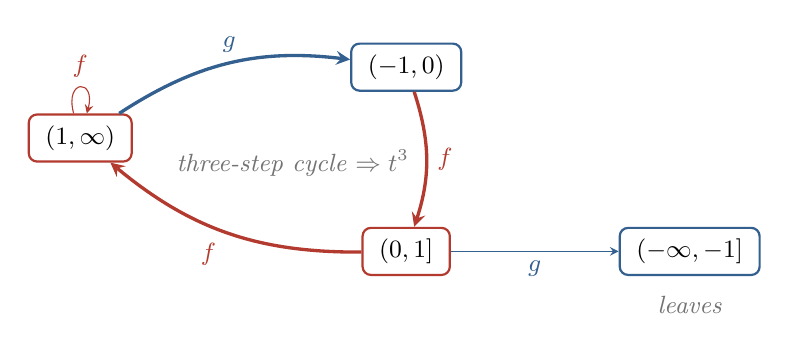
\begin{tikzpicture}[>=stealth,scale=0.9,
  st/.style={draw,rounded corners=3pt,inner xsep=6pt,inner ysep=4pt,font=\small,thick}]
\node[st,draw=fred] (A) at (0,0) {$(1,\infty)$};
\node[st,draw=gblue] (C) at (4.6,1.0) {$(-1,0)$};
\node[st,draw=fred] (B) at (4.6,-1.6) {$(0,1]$};
\node[st,draw=gblue] (D) at (8.6,-1.6) {$(-\infty,-1]$};
\draw[->,gblue,very thick] (A) to[bend left=20] node[above,font=\small]{$g$} (C);
\draw[->,fred,very thick] (C) to[bend left=18] node[right,font=\small]{$f$} (B);
\draw[->,fred,very thick] (B) to[bend left=20] node[below left,font=\small]{$f$} (A);
\path[->,fred] (A) edge[loop above,looseness=7] node[above,font=\small]{$f$} (A);
\draw[->,gblue] (B) -- node[below,font=\small]{$g$} (D);
\node[font=\small\itshape,text=black!55] at (8.6,-2.35) {leaves};
\node[font=\small\itshape,text=black!55] at (3.0,-0.35) {three-step cycle $\Rightarrow t^{3}$};
\end{tikzpicture}
\caption{Child rules between the four sign/size classes (Proposition~\ref{prop:classes}).  The only route
from a $g$-step back into the positives is the three-step cycle
$(1,\infty)\to(-1,0)\to(0,1]\to(1,\infty)$, the structural source of the $t^{3}$ in the recurrence, and a
counting shadow of $(gf)^{3}=\mathrm{id}$ (Remark~\ref{rem:relation}).}
\label{fig:automaton}
\end{figure}

\section{Geodesic words, and completion of the transfer-matrix argument}\label{sec:words}

Reversing $P$-orbits assigns to every rational a canonical geodesic word; we now describe the resulting
language and connect it to the pattern-avoidance argument of \cite{mmz}.

\begin{proposition}[canonical normal forms]\label{prop:normalform}
For $x\in\Q$ let $w(x)$ be the word read along the reversed $P$-orbit of $x$ (empty for $x=0$), as in
Example~\ref{ex:orbit}.  Then:
\begin{enumerate}[(a)]
\item $w(x)$ is admissible at $0$, has endpoint $x$, and has length $|w(x)|=d(x)$;
\item the map $x\mapsto w(x)$ is a bijection from $\Q$ onto the language
\[
\lang \;=\; \{\varepsilon\}\;\cup\;
\Bigl\{\,f^{m_1}g\,f^{m_2}g\cdots f^{m_j}g^{\,\epsilon}\ :\ j\ge1,\ \epsilon\in\{0,1\},\
m_1,\dots,m_{j-1}\ge2,\ m_j\ge1\Bigr\};
\]
\item under this bijection, $\epsilon=1$ exactly for $x<0$, and for $x>0$ the run lengths are the
negative-continued-fraction digits reversed: $(m_1,\dots,m_j)=(c_k,\dots,c_1)$.
\end{enumerate}
\end{proposition}

\begin{proof}
(a) is the upper-bound half of the proof of Theorem~\ref{thm:dist} together with $d=D$.
For (b), (c): evaluation at $0$ recovers $x$ from $w(x)$, so the map is injective.  Let $x>0$ have digits
$(c_1,\dots,c_k)$.  Its orbit is: $c_1$ subtractions, flip, $c_2$ subtractions, flip, \dots, flip, $c_k$
subtractions (Theorem~\ref{thm:hj}); reversing, the word is
$f^{c_k}\,g\,f^{c_{k-1}}\,g\cdots g\,f^{c_1}$, i.e.\ runs $(m_1,\dots,m_j)=(c_k,\dots,c_1)$ with $j=k$,
$\epsilon=0$.  The digit conditions ($c_1\ge1$; $c_i\ge2$ for $i\ge2$) translate exactly to ($m_j\ge1$;
$m_i\ge2$ for $i\le j-1$).  For $x<0$, $w(x)=w(-1/x)\,g$, giving the same runs with $\epsilon=1$.
Conversely every $(j,\epsilon,m_1,\dots,m_j)$ as in the definition of $\lang$ arises from exactly one
valid digit string and sign, by Lemma~\ref{lem:hjexist} and Corollary~\ref{cor:enum}.
\end{proof}

\begin{proposition}[pattern-avoidance description]\label{prop:lang}
$\lang$ equals the set of words over $\{f,g\}$ containing no factor $gg$, containing no factor
$fgfgf$, not beginning with $g$, and not beginning with $fgf$.
\end{proposition}

\begin{proof}
A word with no factor $gg$ and not beginning with $g$ is uniquely of the form
\[
f^{m_1}g\,f^{m_2}g\cdots f^{m_j}g^{\,\epsilon},\qquad m_i\ge1,\ \ \epsilon\in\{0,1\}
\]
(interior $g$'s are single, and a final $g$ is allowed).  Given this shape, a factor $fgfgf$ occurs if and only if some run of length exactly
$1$ is flanked by two $g$'s, each of which has an $f$ beyond it.  The run $m_i$ is flanked by $g$'s iff
$2\le i\le j-1$, or $i=j$ with $\epsilon=1$; but in the latter case there is no letter after the final
$g$.  So ``no factor $fgfgf$'' is equivalent to $m_i\ge2$ for $2\le i\le j-1$.  Similarly the word
begins with $fgf$ iff $m_1=1$ and $j\ge2$.  Hence the four conditions together are equivalent to
$m_i\ge2$ for all $1\le i\le j-1$ and $m_j\ge1$, which is the definition of $\lang$.
\end{proof}

\begin{remark}[what was missing in the Math.SE argument, and how it is now complete]\label{rem:mmz}
The accepted answer \cite{mmz} argued: by $g^{2}=\mathrm{id}$ and $fgfgf=g$ (consequences of the
$\mathrm{PSL}_2(\Z)$ relations), a \emph{minimal} word cannot contain $gg$ or $fgfgf$; and a word may not
begin with $g$ (undefined at $0$) or with $fgf$ (which returns to $0$).  It then counted the words
satisfying these restrictions (the language of Proposition~\ref{prop:lang}, i.e.\ $\lang$) with a
$14$-state automaton, obtaining the generating function $(1+t^{2}-t^{3})/(1-t-t^{3})$.  This computation is
correct, and consistent with Theorem~\ref{thm:main}; what it leaves unproved is that the number of words of
length $n$ in $\lang$ equals $a(n)$.  That is precisely the content of
Propositions~\ref{prop:normalform}--\ref{prop:lang}: \emph{every} word of $\lang$ is geodesic (not merely:
every geodesic avoids the patterns), distinct words of $\lang$ have distinct endpoints, and every rational
is an endpoint.  With these three facts the transfer-matrix computation becomes a second, independent
derivation of Theorem~\ref{thm:main}(a).  (We verified the equality of the three languages, tree words, $\lang$, and the avoidance
language, by exhaustive enumeration through length $14$.)
\end{remark}

\section{Computational verification}\label{sec:verify}

Independently of the proofs, we ran a breadth-first search over $\Q$ in exact integer arithmetic
(fractions stored in lowest terms; the maps preserve lowest terms), reproducing Kimberling's construction
through rank $41$: a total of $14{,}144{,}885$ vertices.  All of the following were checked and hold with
zero anomalies:

\begin{enumerate}[itemsep=1pt]
\item the rank sizes $a(0),\dots,a(41)$ (Table~\ref{tab:counts}) satisfy $a(n)=a(n-1)+a(n-3)$ for
$4\le n\le41$, fail it at $n=3$, and agree with A097333 shifted by one index;
\item at every vertex, the entering edge is $f$ iff the value is positive (Q2);
\item at every vertex $x$: if $x>0$ then $d(x-1)=d(x)-1$; if $x<0$ then $d(-1/x)=d(x)-1$; if $x<-1$ then
$d(x+1)=d(x)-3$; children counts are $(2,1,0)$ for $x>0$, $x\in(-1,0)$, $x\le-1$; no value was produced
twice within a generation;
\item both closed-form rank formulas (Theorems~\ref{thm:hj} and~\ref{thm:reg}) hold at every vertex of
rank $\le32$ ($453{,}457$ vertices, digit strings computed independently of the search);
\item the four-class rules of Proposition~\ref{prop:classes} hold at every rank;
\item the concatenated rows agree term by term, values \emph{and} within-row order, with the
published data of A226247 and A226248 (84 terms of each).
\end{enumerate}

\begin{table}[h]
\centering\small
\begin{tabular}{@{}rr@{\hskip 2.2em}rr@{\hskip 2.2em}rr@{}}
\toprule
$n$ & $a(n)$ & $n$ & $a(n)$ & $n$ & $a(n)$\\
\midrule
0 & 1 & 14 & 148 & 28 & 31{,}224\\
1 & 1 & 15 & 217 & 29 & 45{,}761\\
2 & 2 & 16 & 318 & 30 & 67{,}066\\
3 & 2 & 17 & 466 & 31 & 98{,}290\\
4 & 3 & 18 & 683 & 32 & 144{,}051\\
5 & 5 & 19 & 1{,}001 & 33 & 211{,}117\\
6 & 7 & 20 & 1{,}467 & 34 & 309{,}407\\
7 & 10 & 21 & 2{,}150 & 35 & 453{,}458\\
8 & 15 & 22 & 3{,}151 & 36 & 664{,}575\\
9 & 22 & 23 & 4{,}618 & 37 & 973{,}982\\
10 & 32 & 24 & 6{,}768 & 38 & 1{,}427{,}440\\
11 & 47 & 25 & 9{,}919 & 39 & 2{,}092{,}015\\
12 & 69 & 26 & 14{,}537 & 40 & 3{,}065{,}997\\
13 & 101 & 27 & 21{,}305 & 41 & 4{,}493{,}437\\
\bottomrule
\end{tabular}
\caption{Verified rank sizes $a(n)=|X_n|$ for $0\le n\le41$.}
\label{tab:counts}
\end{table}

\section{Further remarks}\label{sec:remarks}

\begin{remark}[negative integers]
The formulas give pleasant special values.  For $n\ge1$ one checks
$\hj{2,2,\dots,2}$ ($j$ twos) $=(j+1)/j$ by induction, whence $\tfrac1n=\hj{1,2^{\,(n-1)}}$
(meaning one $1$ followed by $n-1$ twos), so $d(1/n)=\bigl(1+2(n-1)\bigr)+n-1=3n-2$ and
\[
d(-n)=3n-1 .
\]
Thus $-1,-2,-3,\dots$ appear at ranks $2,5,8,\dots$, three apart: another visible trace of the
three-step cycle.
\end{remark}

\begin{remark}[sharpness at $n=3$]
The unique failure $a(3)=a(2)+a(0)-1$ is a boundary effect of the root: among words, the automaton of
Section~\ref{sec:words} would admit $fgf$ were it not excluded for returning to $0$ (equivalently: $g$ is
undefined at $0$, so the tree has no vertex ``$\infty$'' and the pattern is banned as a prefix).  This
removes exactly one word of length $3$, matching the coefficient $-t^{3}$ in the numerator of $A(t)$.
\end{remark}

\begin{remark}[positions of the nonpositive entries]
Within Kimberling's concatenated ordering, the nonpositive values occupy positions $n+\mathrm{A005374}(n)$
(Hofstadter's $H$-sequence), a formula recorded in A226249 by G\'omez Calder\'on (2025)
\cite{oeisA226249}.  We have not included a proof here; it is consistent with the class dynamics of
Proposition~\ref{prop:classes}, which shows that the negatives of rank $n$ biject with the positives of
rank $n-1$, so their counting function is governed by the same $t^{3}=t^{2}+1$ substitution structure that
underlies A005374.
\end{remark}

\begin{remark}[variants]
Kimberling's entry also discusses a sibling ordering $S'$ of the rationals built from the same two maps
with different conventions (A226130), for which the analogous count is conjectured at A226136 (cf.\ the
note in \cite{kagey-mse}).  The parent-map method applies verbatim: one first guesses $P$ from small ranks,
then proves the analogues of (D1)--(D4).
\end{remark}

\subsection*{Data and code availability}
The verification script (\texttt{verify.py}, plain Python, $\approx35$ s) and the full solution notes
accompany this document.

\begin{thebibliography}{99}\small

\bibitem{kagey137}
P.~Kagey, \emph{Problem 137}, Open Problem Collection,
\url{https://peterkagey.com/problems/137/} (accessed August 2026).

\bibitem{kagey-mse}
P.~Kagey, \emph{Enumerating all fractions by $x\mapsto x+1$ and $x\mapsto-\frac1x$},
Mathematics Stack Exchange, question 5057812 (April 2025),
\url{https://math.stackexchange.com/q/5057812}.

\bibitem{mmz}
mathmasterzach, \emph{Answer to ``Enumerating all fractions by $x\mapsto x+1$ and
$x\mapsto-\frac1x$''}, Mathematics Stack Exchange (April 2025),
\url{https://math.stackexchange.com/a/5058406}.

\bibitem{oeisA226247}
C.~Kimberling, Sequence A226247 (with A226248, A226249, A226250), in: OEIS Foundation Inc.,
\emph{The On-Line Encyclopedia of Integer Sequences} (2013), \url{https://oeis.org/A226247}.

\bibitem{oeisA226248}
C.~Kimberling, Sequence A226248, in: OEIS, \url{https://oeis.org/A226248}.

\bibitem{oeisA226249}
C.~Kimberling, Sequence A226249 (formula by A.~M.~G\'omez Calder\'on, 2025), in: OEIS,
\url{https://oeis.org/A226249}.

\bibitem{oeisA097333}
OEIS, Sequence A097333, \url{https://oeis.org/A097333}.

\bibitem{oeisA000930}
OEIS, Sequence A000930 (Narayana's cows), \url{https://oeis.org/A000930}.

\bibitem{hirzebruch1953}
F.~Hirzebruch, \emph{\"Uber vierdimensionale Riemannsche Fl\"achen mehrdeutiger analytischer
Funktionen von zwei komplexen Ver\"anderlichen}, Math.\ Ann.\ \textbf{126} (1953), 1--22.

\bibitem{popescu2007}
P.~Popescu-Pampu, \emph{The geometry of continued fractions and the topology of surface
singularities}, in: Singularities in Geometry and Topology 2004, Adv.\ Stud.\ Pure Math.\ \textbf{46},
Math.\ Soc.\ Japan, 2007.

\bibitem{hardywright}
G.~H.~Hardy and E.~M.~Wright, \emph{An Introduction to the Theory of Numbers}, 6th ed.,
Oxford University Press, 2008.

\bibitem{serre1980}
J.-P.~Serre, \emph{Trees}, Springer-Verlag, Berlin--New York, 1980.

\bibitem{alperin1993}
R.~C.~Alperin, \emph{$\mathrm{PSL}_2(\mathbf{Z})=\mathbf{Z}_2*\mathbf{Z}_3$},
Amer.\ Math.\ Monthly \textbf{100} (1993), 385--386.

\end{thebibliography}

\end{document}
